\documentclass[11pt]{article}
\usepackage{fullpage}
\usepackage{setspace}
% load matlab package with ``framed'' and ``numbered'' option.
%\usepackage[framed,numbered,autolinebreaks,useliterate]{mcode}
\usepackage{subfigure}
\usepackage{wrapfig}
\usepackage{graphicx}
\usepackage{cite}
%\usepackage{natbib}
\usepackage{booktabs}
\usepackage{fancyhdr}
\usepackage{amsmath}
\usepackage{amsfonts}
\usepackage{amssymb,amsmath,amsthm}
\usepackage{bm}
\usepackage[english]{babel}
\usepackage{multirow}
\usepackage{enumitem}
\newcommand{\cno}{C/N_0}
\newcommand{\ccoh}{C_{\textrm{coh}}}
\newcommand{\tcoh}{T_{\textrm{coh}}}
\newcommand{\rpm}{\raisebox{.2ex}{$\scriptstyle\pm$}}
\newcommand{\rrpm}{\sbox0{$1$}\sbox2{$\scriptstyle\pm$}
  \raise\dimexpr(\ht0-\ht2)/2\relax\box2 }
  
\title{ASE 372N Laboratory \#1 Report \\In-field data collection with a handheld GPS receiver }
\author{Caleb North} \date{September 8, 2016}

\begin{document}
%\onehalfspace
\maketitle
\section{Abstract}

An error analysis was performed on NMEA 0183 position solutions recorded \textit{in situ} using a Trimble Juno SB handheld GPS receiver. To determine how the WAAS functionality affects performance, the precision and accuracy of the receiver with and without the WAAS capability enabled was assessed. It was found that the inclusion of WAAS did not significantly alter the accuracy, however the horizontal circular error probable (CEP) was reduced by 25\%. To observe how environment impacts performance, data was collected at two separate sites with different horizontal profiles. It was found that the site with less obscura reduced the CEP by 34\%. Furthermore, it was found that measurement precision was  sensitive to satellite geometry. It was shown that a data-set with more satellites in view could reduce the CEP by 38\%.

 
\section{Introduction}

This lab observed how precision and accuracy can be affected by various factors: WAAS functionality enabled/disabled, horizon profile, and GPS constellation geometry. To accomplish this, a Trimble Juno SB handheld GPS receiver, with the SirfTech application installed, was used to record NMEA 0183 position estimates. A total of six 10-minute data collections were carried out at 3 different locations around the University of Texas at Austin. Table \ref{tab:sites} shows when and where (local time) these data collections occurred. 
\\
\begin{table}[h!]
\begin{center}
    \begin{tabular}{  l || c | c| }
    %\hline
Test Name & Location & Start Time\\\hline
\hline
WAAS Enabled    & South Mall & 6:04pm \\\hline
WAAS Disabled   & South Mall & 6:06pm \\\hline
Site 83: Test 1 & 24th St. and San Jacinto Ave. & 8:09pm \\\hline
Site 83: Test 2 & 24th St. and San Jacinto Ave. & 9:52pm \\\hline
Site 56: Test 1 & South-West corner of ECT & 9:21pm \\\hline
Site 56: Test 2 & South-West corner of ECT & 10:18pm \\\hline
    \end{tabular}
\caption{Data-set names, locations, and start times.}
\label{tab:sites}
\end{center}
\end{table}

\pagebreak

%The first data collect occured on the plaza north of the South Mall of the UT South Mall. Durring this collect, the WAAS functionality was enabled. The second data aquisition occured at the same location, directly after the end of the first data collect. The only difference was that the WAAS option was disabled. The rest of the test cases occured with the WAAS capability enabled. The third test occured on the west sidewalk at the intersection of 24th St. and San Jacinto Ave. The data was collected directly over Survey Marker 83, and as such, this test case will be refernced as 'Site 83: Test 1'. The forth test-case occured near the south-west corner of the Engineering Tesching Center (ETC). The collection happened obove Survey Marker 56, and as such, this test case will be reference as 'Site 56:Test 1'. The fift data set was taken over Survey Marker 83 nearly 2 hours after 'Site 83: Test 1', and will be referenced as 'Site 83: Test 2'. The final data-set was recorded at Site 53 an hour after 'Site 53: Test 1', and will be referenced as 'Site 53: Test 2'.

For the data processing, a Matlab function {\tt readNMEAposV3.m} was used to convert the raw NMEA message logs to csv files containing: seconds of day, latitude, longitude, altitude, and number of satellites tracked. Additionally, three Python scripts were written: 1) {\tt lla2ecef.py} converts a position in the LLA frame (Latitude-Longitude-Altitude) to the ECEF frame (Earth Centered Earth Fixed), 2) {\tt ecef2enu.py} calculates the rotation matrix to convert from the Cartesian ECEF frame to the geodetic ENU frame (East-North-Up), and 3) {\tt Lab1.py} is an analysis script tailored for this study, which calculates and plots the means, standard deviations, CEP (circular error probable) for the 2D horizontal, and SEP (spherical error probable) in each frame for each data-set. These scripts can be found in Appendix A.


\section{Results and Analysis}

When the {\tt readNMEAposV3.m} function was fed the test log files, it produced LLA positions. Table \ref{tab:lla} shows the mean values for those positions and SV count.
\\
\begin{table}[h!]
\begin{center}
    \begin{tabular}{  l || c | c | c | c | }
    %\hline
Mean Values & Latitude (rad) & Longitude (rad) & Altitude (m) & Satellites Tracked\\\hline
\hline
WAAS Enabled    & 0.528578693 & -1.70587545 & 178.8 & 9.0 \\\hline
WAAS Disabled   & 0.528578740 & -1.70587534 & 178.8 & 9.3 \\\hline
Site 83: Test 1 & 0.528608035 & -1.70577042 & 159.4 & 8.7 \\\hline
Site 83: Test 2 & 0.528608272 & -1.70577039 & 152.8 & 7.8 \\\hline
Site 56: Test 1 & 0.528655580 & -1.70580959 & 154.1 & 7.9 \\\hline
Site 56: Test 2 & 0.528653904 & -1.70581267 & 204.1 & 6.6 \\\hline
    \end{tabular}
\caption{Mean position values in the LLA frame and mean number of satellites tracked.}
\label{tab:lla}
\end{center}
\end{table}

The script {\tt lla2ecef.py} was used to convert each of the LLA position measurements to ECEF positions. The average ECEF position for each data-set was computed and is shown in Table \ref{tab:ecef}
\\
\begin{table}[h!]
\begin{center}
    \begin{tabular}{  l || c | c | c | c | }
    %\hline
Mean Values & X (Km) & Y (Km) & Z (Km) & Satellites Tracked\\\hline
\hline
WAAS Enabled    & -742.365067 & -5462.31250 &  3197.81682 & 9.0 \\\hline
WAAS Disabled   & -742.364432 & -5462.31243 &  3197.81707 & 9.3 \\\hline
Site 83: Test 1 & -741.776405 & -5462.28071 &  3197.96797 & 8.7 \\\hline
Site 83: Test 2 & -741.775362 & -5462.27429 &  3197.96592 & 7.8 \\\hline
Site 56: Test 1 & -741.969267 & -5462.09619 &  3198.22607 & 7.9 \\\hline
Site 56: Test 2 & -741.992631 & -5462.14200 &  3198.24210 & 6.6 \\\hline
    \end{tabular}
\caption{Mean position values in the ECEF frame and mean number of satellites tracked.}
\label{tab:ecef}
\end{center}
\end{table}

Removing the average from the ECEF positions resulted in a collection of ECEF residuals. The residuals where then converted to ENU and the standard error metrics where calculated (See Appendix A). Table \ref{tab:stats} shows error metrics for position and number of tracked satellites for each data set.
\\
\begin{table}[h!]
\begin{center}
    \begin{tabular}{  l || c | c | c | c | c | c | }
    %\hline
  & $\sigma_{East}$ (m) & $\sigma_{North}$ (m) & $\sigma_{Up}$ (m) & CEP (m) & SEP (m) & Satellites Tracked \\\hline
  \hline
WAAS Enabled    &  0.48  & 0.61 &  1.82 & 0.65 & 1.52 & 9.0 \\\hline
WAAS Disabled   &  0.70  & 0.75 &  2.19 & 0.86 & 1.86 & 9.3 \\\hline
Site 83: Test 1 &  1.54  & 0.95 &  3.10 & 1.50 & 2.76 & 8.7 \\\hline
Site 83: Test 2 &  2.12  & 2.37 &  6.18 & 2.65 & 5.34 & 7.8 \\\hline
Site 56: Test 1 &  1.35  & 2.36 &  3.63 & 2.27 & 3.49 & 7.9 \\\hline
Site 56: Test 2 &  2.43  & 1.01 &  7.44 & 2.20 & 6.07 & 6.6 \\\hline
    \end{tabular}
\caption{Error metrics for each data-set.}
\label{tab:stats}
\end{center}
\end{table}

By inspection, it is observed that data-sets which were tracking more satellites appear to have less statistical error, i.e. more precision.



\subsection{WAAS}

The WAAS satellite provides differential corrections to the GPS satellites. So, it is expected that the use of the WAAS functionality would provide a better solution, i.e. more accuracy and precision. This section will determine how much of an improvement was observed in the measurements. Figure \ref{fig:WAAS} shows the ENU residuals for the receiver with and without the WAAS option enabled.

\begin{figure}[h]
\begin{center}
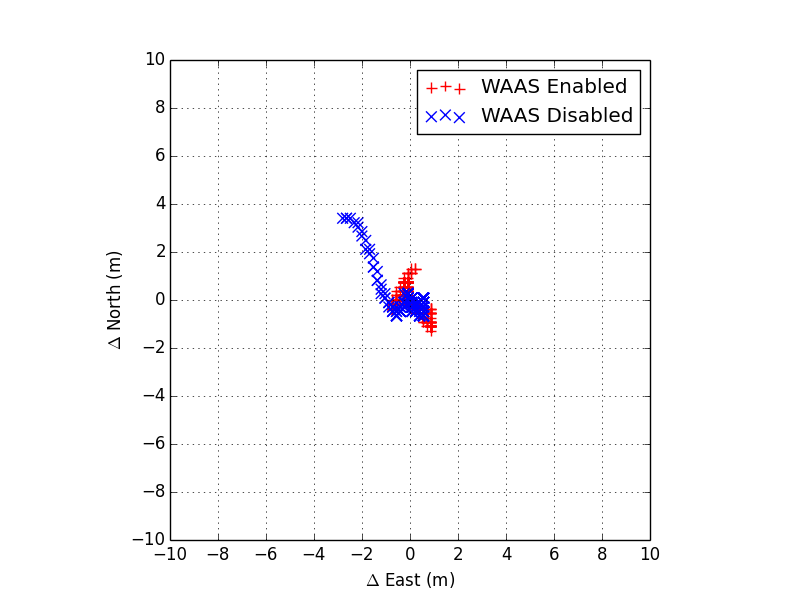
\includegraphics[width=0.75\textwidth]{ENU-residual-WAAS.png}
\end{center}
\caption{ENU residuals with and without WAAS enabled.}
\label{fig:WAAS}
\end{figure}


Table \ref{tab:WAAS} displays the error metrics, comparing the WAAS enable/disable data-sets. From inspection, it is observed that enabling the WAAS functionality reduced the CEP by 25\%.

\begin{table}[h!]
\begin{center}
    \begin{tabular}{  l || c | c | c | c | c | }
    %\hline
 & $\sigma_{East}$ (m) & $\sigma_{North}$ (m) & $\sigma_{Up}$ (m) & CEP (m) & SEP (m) \\\hline\hline
WAAS Enabled    &  0.48  & 0.61 &  1.82 & 0.65 & 1.52 \\\hline
WAAS Disabled   &  0.70  & 0.75 &  2.19 & 0.86 & 1.86 \\\hline
    \end{tabular}
\caption{Error metrics with and without WAAS enabled.}
\label{tab:WAAS}
\end{center}
\end{table}

 

\subsection{Satellite Geometry}

As time progresses the GPS satellites sweep out tracks in the sky. This means that the geometry of the GPS constellation is ever-changing. A consequence of this phenomenon, is that the precision GPS position measurements is also changing, especially in urban canyons which can be found throughout the UT campus. Two data collects where taken nearly 2hrs apart. The analysis presented in this section is intended to determine how the precision is affected.

\vspace{2mm}
Figure \ref{fig:mustang} shows the position residuals, with respect to the mean, on the position estimates in the LLA frame on the left, and ENU frame on the right. A cursory comparison shows that the two frames have similar behavior, which is to be expected.

\begin{figure}[h]
\begin{center}$
\begin{array}{ccc}\hspace{-8em}
 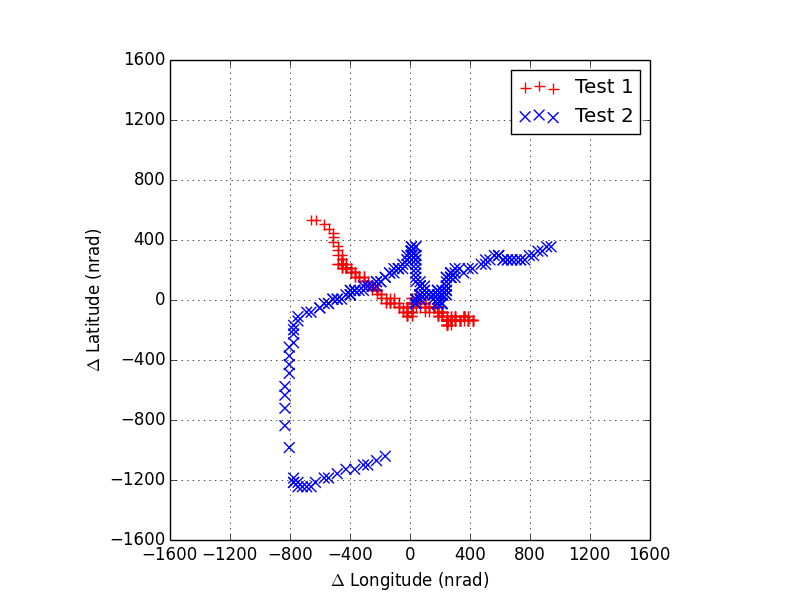
\includegraphics[width=0.75\textwidth]{LLA-residuals-Mustang.png} &\hspace{-5em}
 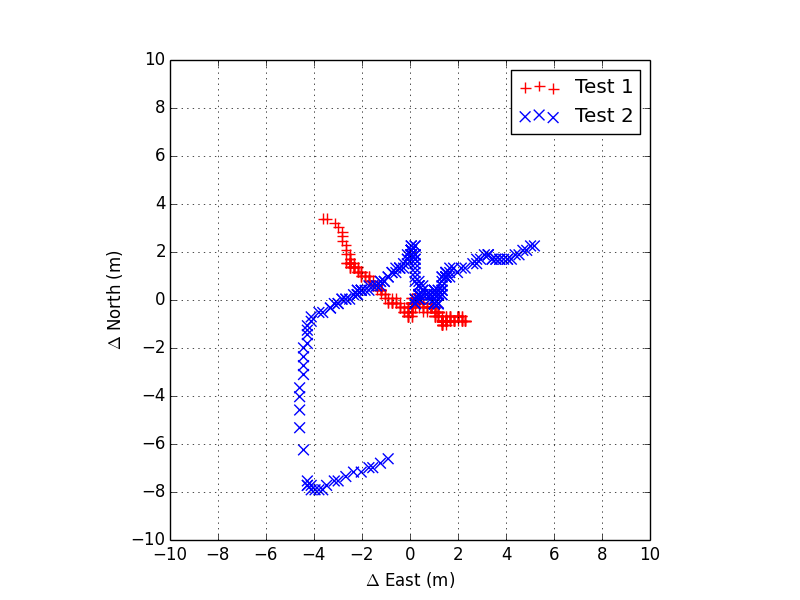
\includegraphics[width=0.75\textwidth]{ENU-residuals-Mustang.png}
\end{array}$
\end{center}
\caption{Residuals from the mean for Test 1 and 2 in the LLA frame (left) and ENU frame (right).}
\label{fig:mustang}
\end{figure}

Table \ref{tab:mustang} displays the error metrics, comparing data-sets collected from the same location, but 2 hours apart. From inspection, the site with less obscura reduced the CEP by 34\%. The precision of the receiver can be interpreted to be 

\begin{table}[h!]
\begin{center}
    \begin{tabular}{  l || c | c | c | c | c | c |}
    %\hline
 & $\sigma_{East}$ (m) & $\sigma_{North}$ (m) & $\sigma_{Up}$ (m) & CEP (m) & SEP (m) & Rx's Error (m)\\\hline
 \hline
Site 83: Test 1 & 1.54 & 0.95 & 3.10 & 1.50 & 2.76 & 3.5\\\hline
Site 83: Test 2 & 2.12 & 2.37 & 6.18 & 2.65 & 5.34 & 6.8\\\hline
    \end{tabular}
\caption{Table illustrates...}
\label{tab:mustang}
\end{center}
\end{table}

When focusing on Site 83: Test 1, we find the standard deviation of the vertical height residuals to be on the order of 3m, while the CEP of the horizontal is 1.5m. This indicates that the vertical error is twice as much as the horizontal, which can be understood with the realization that the vertical component only has satellites in the zenith. Another way of stating this is that the VDOP is larger than the HDOP. The SEP is reported to be 2.76m, while the receiver's internal error estimate was recorded to be 3.5m. This could be understood if the internal estimator is using the 3D-RMS which can be approximated as: 3D-RMS = 1.3$\times$SEP = 3.6m. This would give very good agreement with the computed value.


Google Earth was used to overlay the position measurements (LLA) with imagery. Site 83's mark is indicated in the figure by a red circle. The accuracy of Google Earth's rendering appears to be on the order of 3m.

\begin{figure}[h]
\begin{center}
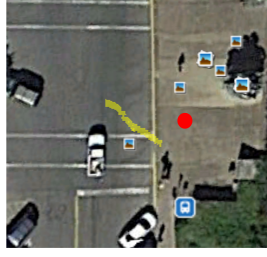
\includegraphics[width=0.5\textwidth]{googleEarth}
\end{center}
\caption{Google Earth generated imagery showing Site 83 (red) with Test 1 data overlaid (yellow).}
\label{fig:googleEarth}
\end{figure}

\subsection{Horizon Profile}

Sky visibility is is crucial for achieving high precision with GPS receivers. This section will observe how the measurement precision behaves, when measurements are taken at two different locations, each with unique horizon profiles. Table \ref{tab:horizon} shows a comparison of two site with different sky-lines. From inspection, Site 83 has a 38\% reduction in CEP when compared to Site 56. It is also apparent that the site with more precision is tracking 1 more SV for the majority of the data-set.

\begin{table}[h!]
\begin{center}
    \begin{tabular}{  l || c | c | c | c | c | c | }
    %\hline
  & $\sigma_{East}$ (m) & $\sigma_{North}$ (m) & $\sigma_{Up}$ (m) & CEP (m) & SEP (m) & Satellites Tracked \\\hline
  \hline
Site 83: Test 1 &  1.54  & 0.95 &  3.10 & 1.50 & 2.76 & 8.7 \\\hline
Site 56: Test 1 &  1.35  & 2.36 &  3.63 & 2.27 & 3.49 & 7.9 \\\hline
    \end{tabular}
\caption{Table illustrates...}
\label{tab:horizon}
\end{center}
\end{table}

Figure \ref{fig:googleMaps} shows how Google Maps was used to estimate a distance of 370m between Site 83 and Site 56. While, the magnitude of the difference in ECEF position between 'Site 83: Test 1' and Site 56: Test 1' indicates that the separation distance is 371m.

\begin{figure}[h]
\begin{center}
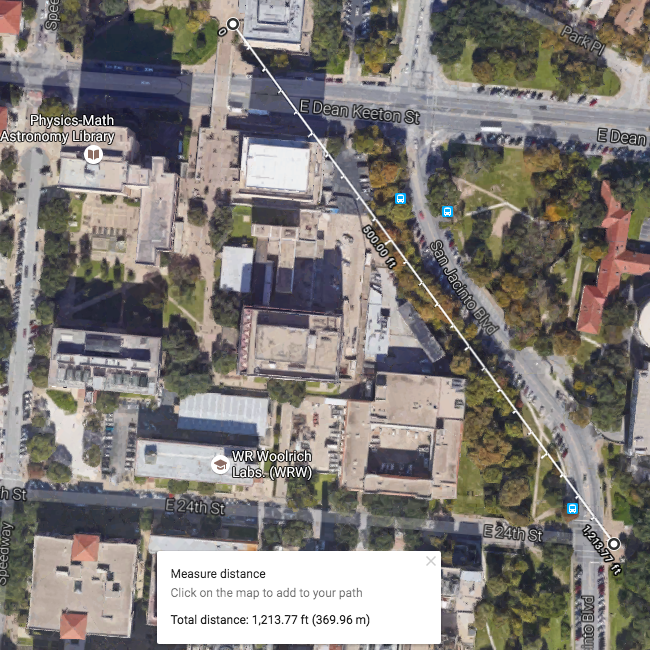
\includegraphics[width=0.5\textwidth]{googleMaps}
\end{center}
\caption{.}
\label{fig:googleMaps}
\end{figure}







\section{Conclusion}

A quantitative analysis was performed on NMEA 0183 position estimates taken from a Trimble Juno SB handheld GPS receiver. To determine how the WAAS functionality affects performance, the precision and accuracy of the receiver with and without the WAAS capability enabled was assessed. It was found that the inclusion of WAAS did not significantly alter the accuracy, however the circular error probable (CEP) for the horizon was reduced by 25\%. Data was collected at two separate sites with different horizontal profiles to observe how environment impacts performance. It was found that the site with more sky-coverage reduced the CEP by 34\%. Furthermore, it was found that precision was sensitive to satellite geometry. It was shown that a site could reduce the CEP by 38\% by just have 1 more satellite in view. 


\bibliographystyle{ieeetr}
\bibliography{pangea}  

\section{Appendix A}
Scripts will be attached individually.
\end{document}
